\subsection{Implementation Strategy}
\label{sec:fitsImplementation}

\begin{figure}[t]
\begin{center}
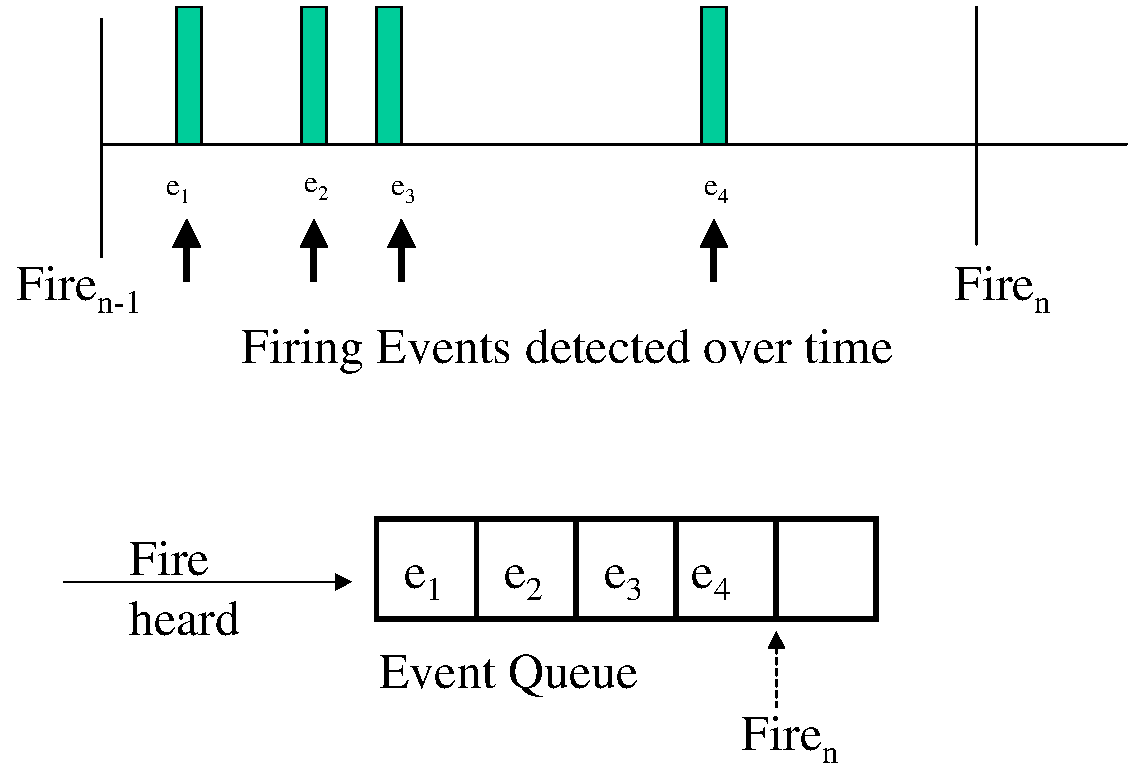
\includegraphics[width=0.9\hsize]{./figures/sortedQueue.pdf}
\end{center}
\caption{{\small {\bf Event Processing: Detected events are stored in a queue sorted by their arrival times and processed at a given time.}}} 
\label{fig:sortedQueue}
\end{figure}

\noindent
In order to address the aforementioned delays introduced by the wireless
sensor network environment, we design an implementation strategy to virtualize time. \\

\noindent
{\bf Processing Events}  \\
In our system each firing event is characterized by 
two messages, the firing message itself and a delay message. 
A firing message contains the sender's local time at
the time it queued the firing message to be sent. A delay message
contains a second timestamp, again using the sender's local
time. The difference between these times represents how long ago the
firing was meant to have occurred. A receiver can then record a firing
event in its own local time by simply subtracting the delay from the
reception time. Each node is assigned a sorted queue to store
detected firing events. The resulting firing event, stored in local time,
is added to the node's sorted queue to be processed later.
All firing events received in one cycle, i.e. received upto a certain amount of 
\emph{idle} time are stored in this queue.  Thus each node remains idle
for a certain period of $\delta(t)$ time, during which it receives and records
firing events. When this idle period is over, the node begins to process the queued events.
Fig.~\ref{fig:sortedQueue} illustrates the queue-based approach of storing
and processing firing events.

Each time a node fires, the next time it will fire can be computed
based on the firing events it detected thus far that are 
stored in the sorted queue.

The tradeoff of the virtualized time strategy is that the response to firing events
is no longer in real time. Firing events detected impact the next firing cycle rather than
the current one. For instance in the first cycle, there are no events in the queue.
Thus, we program the nodes to remain idle by simply storing and processing the events
they detect during this first cycle.

We take a moment to digress to detail a caveat introduced by our hardware
platform. The radio stack on the MicaZ sensor motes, CC2420, does not
permit including the delay message in the same packet as the firing message.
Therefore, two messages are necessary.\\

\noindent
{\bf Computing Next Firing Time}  \\
A node moves closer to firing based on two factors: detecting a firing
and the passing of time. When a firing event is dequeued, the amount of 
elapsed time since the last event recorded is noted.
The represents the time spent waiting without detecting any event. 
This interval is added to the current time, and the magnitude of the jump
on the firing function is computed. This jump is added to the node's 
current time.

In order to implement this, two notions of time need to be tracked:
wall clock time,  which represents the time elapsed between processing
events, as well as the value on the x-axis of the node's current
position on the firing function. \\

\noindent
{\bf 'Ignore-period' For Addressing Pulse Additivity Issues}  \\
Initial experiments showed that on a 15 nodes fully connected graph,
the nodes split into two groups where each individual group achieves synchronicity
amongst its members, but does not achieve synchronicity with the other group.
We believe one reason could be that the additive effect of multiple firings
from the neighboring group is preventing the group from synchronizing with
that group. In order to correct for this \emph{additivity} issue, we 
introduce an \emph{ignore-period} which characterizes the amount of time
during which a node just drops detected events rather than processing
them or storing them in a queue.  Since the ignore-period period may
not be the best solution for the additivity issue, we have implemented
it in a select number of experiments, to determine its effectiveness
in addressing the pulse additivity issues.

